\documentclass{article}
\usepackage[utf8]{inputenc}
\usepackage[italian]{babel}
\usepackage{amsmath}
\usepackage{amssymb}
\usepackage{siunitx}
\usepackage{tabularray}
\usepackage{graphicx}
\usepackage{float}
% \usepackage{minted}
\usepackage[bottom]{footmisc}
\usepackage[page]{appendix}
\newcommand*{\diam}{\varnothing}
\newcommand*{\best}[1]{{#1}_\text{best}}
\newcommand*{\bestp}[1]{{\left(#1\right)}_\text{best}}
\newcommand*{\pbest}[1]{\left({#1}_\text{best}\right)}
\newcommand*{\pbestp}[1]{\left({\left(#1\right)}_\text{best}\right)}
\newcommand*{\errrel}[1]{\frac{\delta #1}{{#1}_\text{best}}}
\title{
  Laboratorio di Fisica 1\\
  R7: Misura di $\left|\vec{g}\right|$ mediante pendolo fisico
}
\author{Gruppo 15: Bergamaschi Riccardo, Graiani Elia, Moglia Simone}
\date{05/03/2024 – 12/03/2024}
\makeindex
\begin{document}

\maketitle

\begin{abstract}
  Il gruppo di lavoro ha misurato il modulo del campo gravitazionale locale
  ($g$) studiando il moto oscillatorio di un pendolo fisico.
\end{abstract}

\setcounter{section}{-1}
\section{Materiali e strumenti di misura utilizzati}
\begin{center}
  \begin{tblr}{
    width=\textwidth,
    colspec={ X[2,m,j]X[1,m,c]X[1,m,c]X[1,m,c] },
    vlines,
}
    \hline
    \textbf{Strumento di misura} & \textbf{Soglia} & \textbf{Portata} & \textbf{Sensibilità} \\
    \hline
    Sensore di rotazione & $\qty{0.002}{rad}$ & N./A. & $\qty{0.002}{rad}$ \\
    \hline[dashed]
    Cronometro & $\qty{0.001}{s}$ & N./A. & $\qty{0.001}{s}$ \\
    \hline[dashed]
    Micrometro ad asta filettata & $\qty{0.01}{mm}$ & $\qty{25.00}{mm}$ & $\qty{0.01}{mm}$ \\
    \hline[dashed]
    Calibro ventesimale & $\qty{0.05}{mm}$ & $\qty{150.00}{mm}$ & $\qty{0.05}{mm}$ \\
    \hline[dashed]
    Metro & $\qty{0.1}{cm}$ & $\qty{300.0}{cm}$ & $\qty{0.1}{cm}$ \\
    \hline[dashed]
    Bilancia di precisione & $\qty{0.01}{g}$ & $\qty{6200.00}{g}$ & $\qty{0.01}{g}$ \\
    \hline
  \end{tblr}
  \begin{tblr}{
    width=\textwidth,
    colspec={ X[m,j]X[3,m,j] },
    vlines,
  }
    \hline
    \textbf{Altro} & \textbf{Descrizione/Note} \\
    \hline
    Asta e rotore & {
      L'asta, fissata ortogonalmente al rotore,
      è libera di ruotare attorno ad un suo estremo.
      Il rotore è invece innestato del sensore di rotazione.
    } \\
    \hline[dashed]
    {Tre cilindri \\ (con masse e raggi distinti)} & {
      Di masse e raggi distinti,
      presentano un foro centrale lungo l'asse di
      simmetria. \\ Li indicheremo con $A$, $B$ e $C$.
      } \\
    \hline
  \end{tblr}
\end{center}

\pagebreak
\section{Esperienza e procedimento di misura}

\emph{
  \textbf{Definizione.} Con il termine “\emph{configurazione}”
  indicheremo d'ora in poi l'insieme delle posizioni di una
  qualunque combinazione di cilindri lungo l'asta, misurate
  rispetto all'estremo fissato al rotore.\footnote{
    Più formalmente, diremo “configurazione” un insieme $\Gamma$
    di coppie ordinate $\gamma$ della forma
    $(i,d)$, dove $i\in\left\{A,B,C\right\}$
    è un cilindro e $d$ è la sua distanza dall'estremo fissato
    al rotore. Ovviamente non è possibile ripetere $i$ in elementi
    distinti della configurazione, perché ciò non avrebbe
    significato fisico.
  }
}

\begin{enumerate}
  \item
    Misuriamo le masse dei cilindri con la bilancia di precisione,
    i rispettivi diametri (interni ed esterni) con il calibro
    ventesimale e le altezze con il micrometro ad asta filettata.
  \item
    Mediante il metro a nastro misuriamo la lunghezza dell'asta e,
    servendoci del micrometro, i diametri di asta e rotore.
  \item
    Ripetiamo 9 volte i seguenti passi:
  \begin{enumerate}
    \item
      Scelta arbitrariamente una configurazione $\Gamma$,
      fissiamo all'asta i cilindri coinvolti,
      servendoci del foro centrale.
      Misuriamo poi, mediante il metro a nastro,
      le posizioni dei cilindri lungo l'asta
      rispetto al suo estremo fisso.
    \item
      Servendoci dell'apposito programma, avviamo
      l'acquisizione dell'angolo in funzione del tempo
      ($\theta(t)$, lo definiremo formalmente più avanti).
    \item
      Inclinando l'asta rispetto alla sua posizione di equilibrio
      di un angolo prefissato $\theta_0$,
      sufficientemente piccolo\footnote{
Questa condizione sull'angolo $\theta_0$ ci permette di approssimare
$\sin(\theta) \sim \theta\quad\forall \theta \in [-\theta_0, \theta_0]$.
      }, diamo inizio al moto del pendolo.
      Acquisiamo dati fino all'arresto del moto.
  \end{enumerate}
\end{enumerate}

\section{Analisi dei dati raccolti e conclusioni}
\emph{\textbf{Nota.}
Avendo valutato gli errori sulle grandezze misurate direttamente
come piccoli, casuali e indipendenti, per svolgere ogni calcolo
abbiamo utilizzato la tradizionale propagazione degli errori.
}

\subsection{Misura di $\left|\vec{g}\right|$}

Scegliamo un sistema di riferimento cilindrico, con
origine all'intersezione fra l'asse di rotazione e il piano,
ad esso perpendicolare, contenente il centro di massa, versore $\hat{r}$
parallelo a $\vec{g}$ e versore $\hat{k}$ diretto lungo l'asse di
rotazione del sistema.

La posizione del centro di massa del pendolo fisico sarà allora descritta
da $\vec{r}_\text{CM} = (r_\text{CM},\theta,z)$ con $z=0$, dove $\theta$
è lo spostamento angolare rispetto alla posizione di equilibrio.

Vale la seconda equazione cardinale della dinamica:
\[\sum\tau^\text{ext}_z = \dot{L}_z = I_z^\text{\,tot} \ddot{\theta}\]

\vspace{2mm}
\emph{
  \textbf{Nota.} In questa sezione abbiamo trascurato la presenza di
  attriti, ma chiaramente gli attriti ci sono e il moto è smorzato.
  Nella sezione successiva tratteremo proprio questo fenomeno,
  determinando, alla luce dei dati raccolti, quanto influisca
  sul valore di $g$.
}
\vspace{2mm}

Poiché l'unica forza esterna al sistema che compie un momento lungo
$\hat{k}$ è la forza peso, si ha:
\[
  \sum\vec{\tau}^\text{\,ext}_z =
  \vec{r}_\text{CM}\times M\vec{g} = -Mg\,r_\text{CM}\sin(\theta)\hat{k}.
\]

L'equazione differenziale che descrive il moto del centro di massa
del pendolo fisico sarà allora:
\[ \ddot{\theta} = -\frac{Mg\,r_\text{CM}}{I_z^\text{tot}}\sin(\theta) \]

È possibile semplificare il modello fisico approssimando
$\sin(\theta)\simeq\theta$. Il gruppo di lavoro ha ritenuto
valida questa operazione solo quando
\[\left|\theta_0-\sin(\theta_0)\right| < \delta\theta\]

Essendo, nel nostro caso, $\delta\theta=\qty{0.02}{rad}$, abbiamo scelto
$\theta_0^\text{max} = \qty{0.49}{rad}$. Infatti:
\[
  \qty{0.49}{rad} - \sin(\qty{0.49}{rad}) \simeq \qty{0.019}{rad}
  \qquad
  \qty{0.50}{rad} - \sin(\qty{0.50}{rad}) \simeq \qty{0.021}{rad}
\]

Prima di prendere ogni misura, il gruppo di lavoro si è assicurato
che $\theta_0$ soddisfacesse abbondantemente la condizione
$\theta_0<\theta_0^\text{max}$.

L'equazione differenziale semplificata è allora:
\[ \ddot{\theta} = -\frac{Mg\,r_\text{CM}}{I_z^\text{tot}} \theta \]

Questa equazione descrive un moto armonico. Le soluzioni sono infatti
del tipo:
\[
  \theta(t) = \theta_0\cos(\omega t)
  \quad\text{dove}\quad
  \omega = \sqrt{\frac{Mg\,r_\text{CM}}{I_z^\text{tot}}}\quad\text{è detta “pulsazione”}.
\]

Possiamo tuttavia facilmente esprimere $\omega$ in funzione del periodo
$T$ del moto oscillatorio, più semplice da calcolare dai dati acquisiti.
Vale infatti:
\[
  \omega = \frac{2\pi}{T}
  \qquad\text{e quindi}\qquad
  \frac{I_z^\text{tot}}{Mr_\text{CM}} = g \frac{T^2}{4\pi^2}
\]

%\subsubsection{Il calcolo di $I_z^\text{tot}$ e $Mr_\text{CM}$}
La formula utilizzata per il calcolo di $I_z^\text{tot}$ riflette la composizione
del sistema, sfruttando la proprietà additiva del momento d'inerzia:
\[I_z^\text{tot} = I_{z,\text{rotore}} + I_{z,\text{asta}} + \sum_{\gamma\in\Gamma} I_{z,\gamma}\]

Chiaramente, per calcolare i momenti d'inerzia rispetto all'asse di
rotazione è necessario applicare il teorema di Huygens-Steiner
a quelli calcolati sui rispettivi centri di massa:
\[
  I_{z,\text{asta}} = I_\text{CM,asta} + m_\text{asta}\left(\frac{L_\text{asta} + \diam_\text{rotore}}{2}\right)^2
\]\[
  I_{z,(i,d)} = I_{\text{CM},i} + m_i\left(d + \frac{h_i - \diam_\text{rotore}}{2}\right)^2\qquad\forall(i,d)\in\Gamma
\]

Per calcolare il termine $M r_\text{CM}$, si osservi che, per la
definizione di posizione del centro di massa, la massa totale si
semplifica:
\[\begin{aligned}
  Mr_\text{CM} &= M\cdot \frac{1}{M}\left(
    m_\text{rotore}\cdot 0 + m_\text{asta} r_\text{CM,asta} +
    \sum_{(i,d)\in\Gamma}{m_i r_{\text{CM},i}}
  \right) \\&= m_\text{asta}\left(\frac{L_\text{asta} + \diam_\text{rotore}}{2}\right) +
    \sum_{(i,d)\in\Gamma}{m_i \left(d + \frac{h_i - \diam_\text{rotore}}{2}\right)}
\end{aligned}\]

Di seguito riportiamo le misure, dirette e indirette, utilizzate per il calcolo dei momenti d'inerzia:

\begin{center}
  \begin{tblr}{ |c|c|c|c|c| }
    \hline
    Oggetto & $l\;\;(\unit{cm})$ & $\diam\;\;(\unit{mm})$ & $m\;\;(\unit{g})$ & $I_\text{CM}\;\;(10^{-5}\,\unit{kg\,m^2})$ \\
    \hline
    Asta & $60.0\pm0.1$ & $5.94\pm0.01$ & $45.82\pm0.01$ & $568.5\pm1.5$ \\
    \hline[dashed]
    Rotore & N./A. & $13.41\pm0.01$ & $22.4\pm0.1^*$ & $0.058\pm0.001^*$ \\
    \hline
  \end{tblr}
\end{center}\begin{center}
  \begin{tblr}{ |c|c|c|c|c|c| }
    \hline
    $i$ & $m_i\;\;(\unit{g})$ & $d_i^\text{\,ext}\;\;(\unit{mm})$ & $d_i^\text{\,int}\;\;(\unit{mm})$ & $h_i\;\;(\unit{mm})$ & $I_{\text{CM},i}\;(\unit{mg\,m^2})$ \\
    \hline
    A & $115.95\pm0.01$ & $29.95 \pm 0.05$ & $6.20 \pm 0.05$ & $19.93 \pm 0.01$ & $10.62\pm0.03$ \\
    \hline[dashed]
    B & $115.86\pm0.01$ & $29.95 \pm 0.05$ & $6.20 \pm 0.05$ & $19.89 \pm 0.01$ & $10.59\pm0.03$\\
    \hline[dashed]
    C & $71.46\pm0.01$ & $29.95 \pm 0.05$ & $6.20 \pm 0.05$ & $12.08 \pm 0.01$ & $5.047\pm0.018$\\
    \hline
\end{tblr}
\end{center}

\emph{$[^*]$ Valori dati}

\pagebreak
%\subsubsection{La misura di $T$}
Il periodo dell'oscillazione è stato misurato individuando $N+1$ zeri
consecutivi di $\theta(t)$, diciamo $\left\{t_0,t_1,\dots,t_N\right\}$.
Allora, poiché tra uno zero e l'altro corre metà periodo, è possibile
calcolare $T$ in questo modo: $T = \frac{2}{N}(t_N - t_0)$

Il gruppo di lavoro ha scelto $N$ di volta in volta, in modo tale che
fosse proporzionale al numero di oscillazioni compiute dal pendolo
prima di fermarsi. Complessivamente, $N$ ha assunto valori da $30$ a
$180$.

\vspace{2mm}
%\subsubsection{Il calcolo di $g$}

Come descritto sopra, il gruppo di lavoro ha calcolato, per ogni
configurazione $\Gamma$,
i valori di $\frac{I_z^\text{tot}}{Mr_\text{CM}}$
e $\frac{T^2}{4\pi^2}$, riportati nel grafico seguente.

Come è possibile osservare dalla relazione che le lega, la dipendenza
tra queste due grandezze è lineare: questo ci permette di determinare
il valore di $g$ come coefficiente angolare di una retta di regressione.

\begin{figure}[H]
  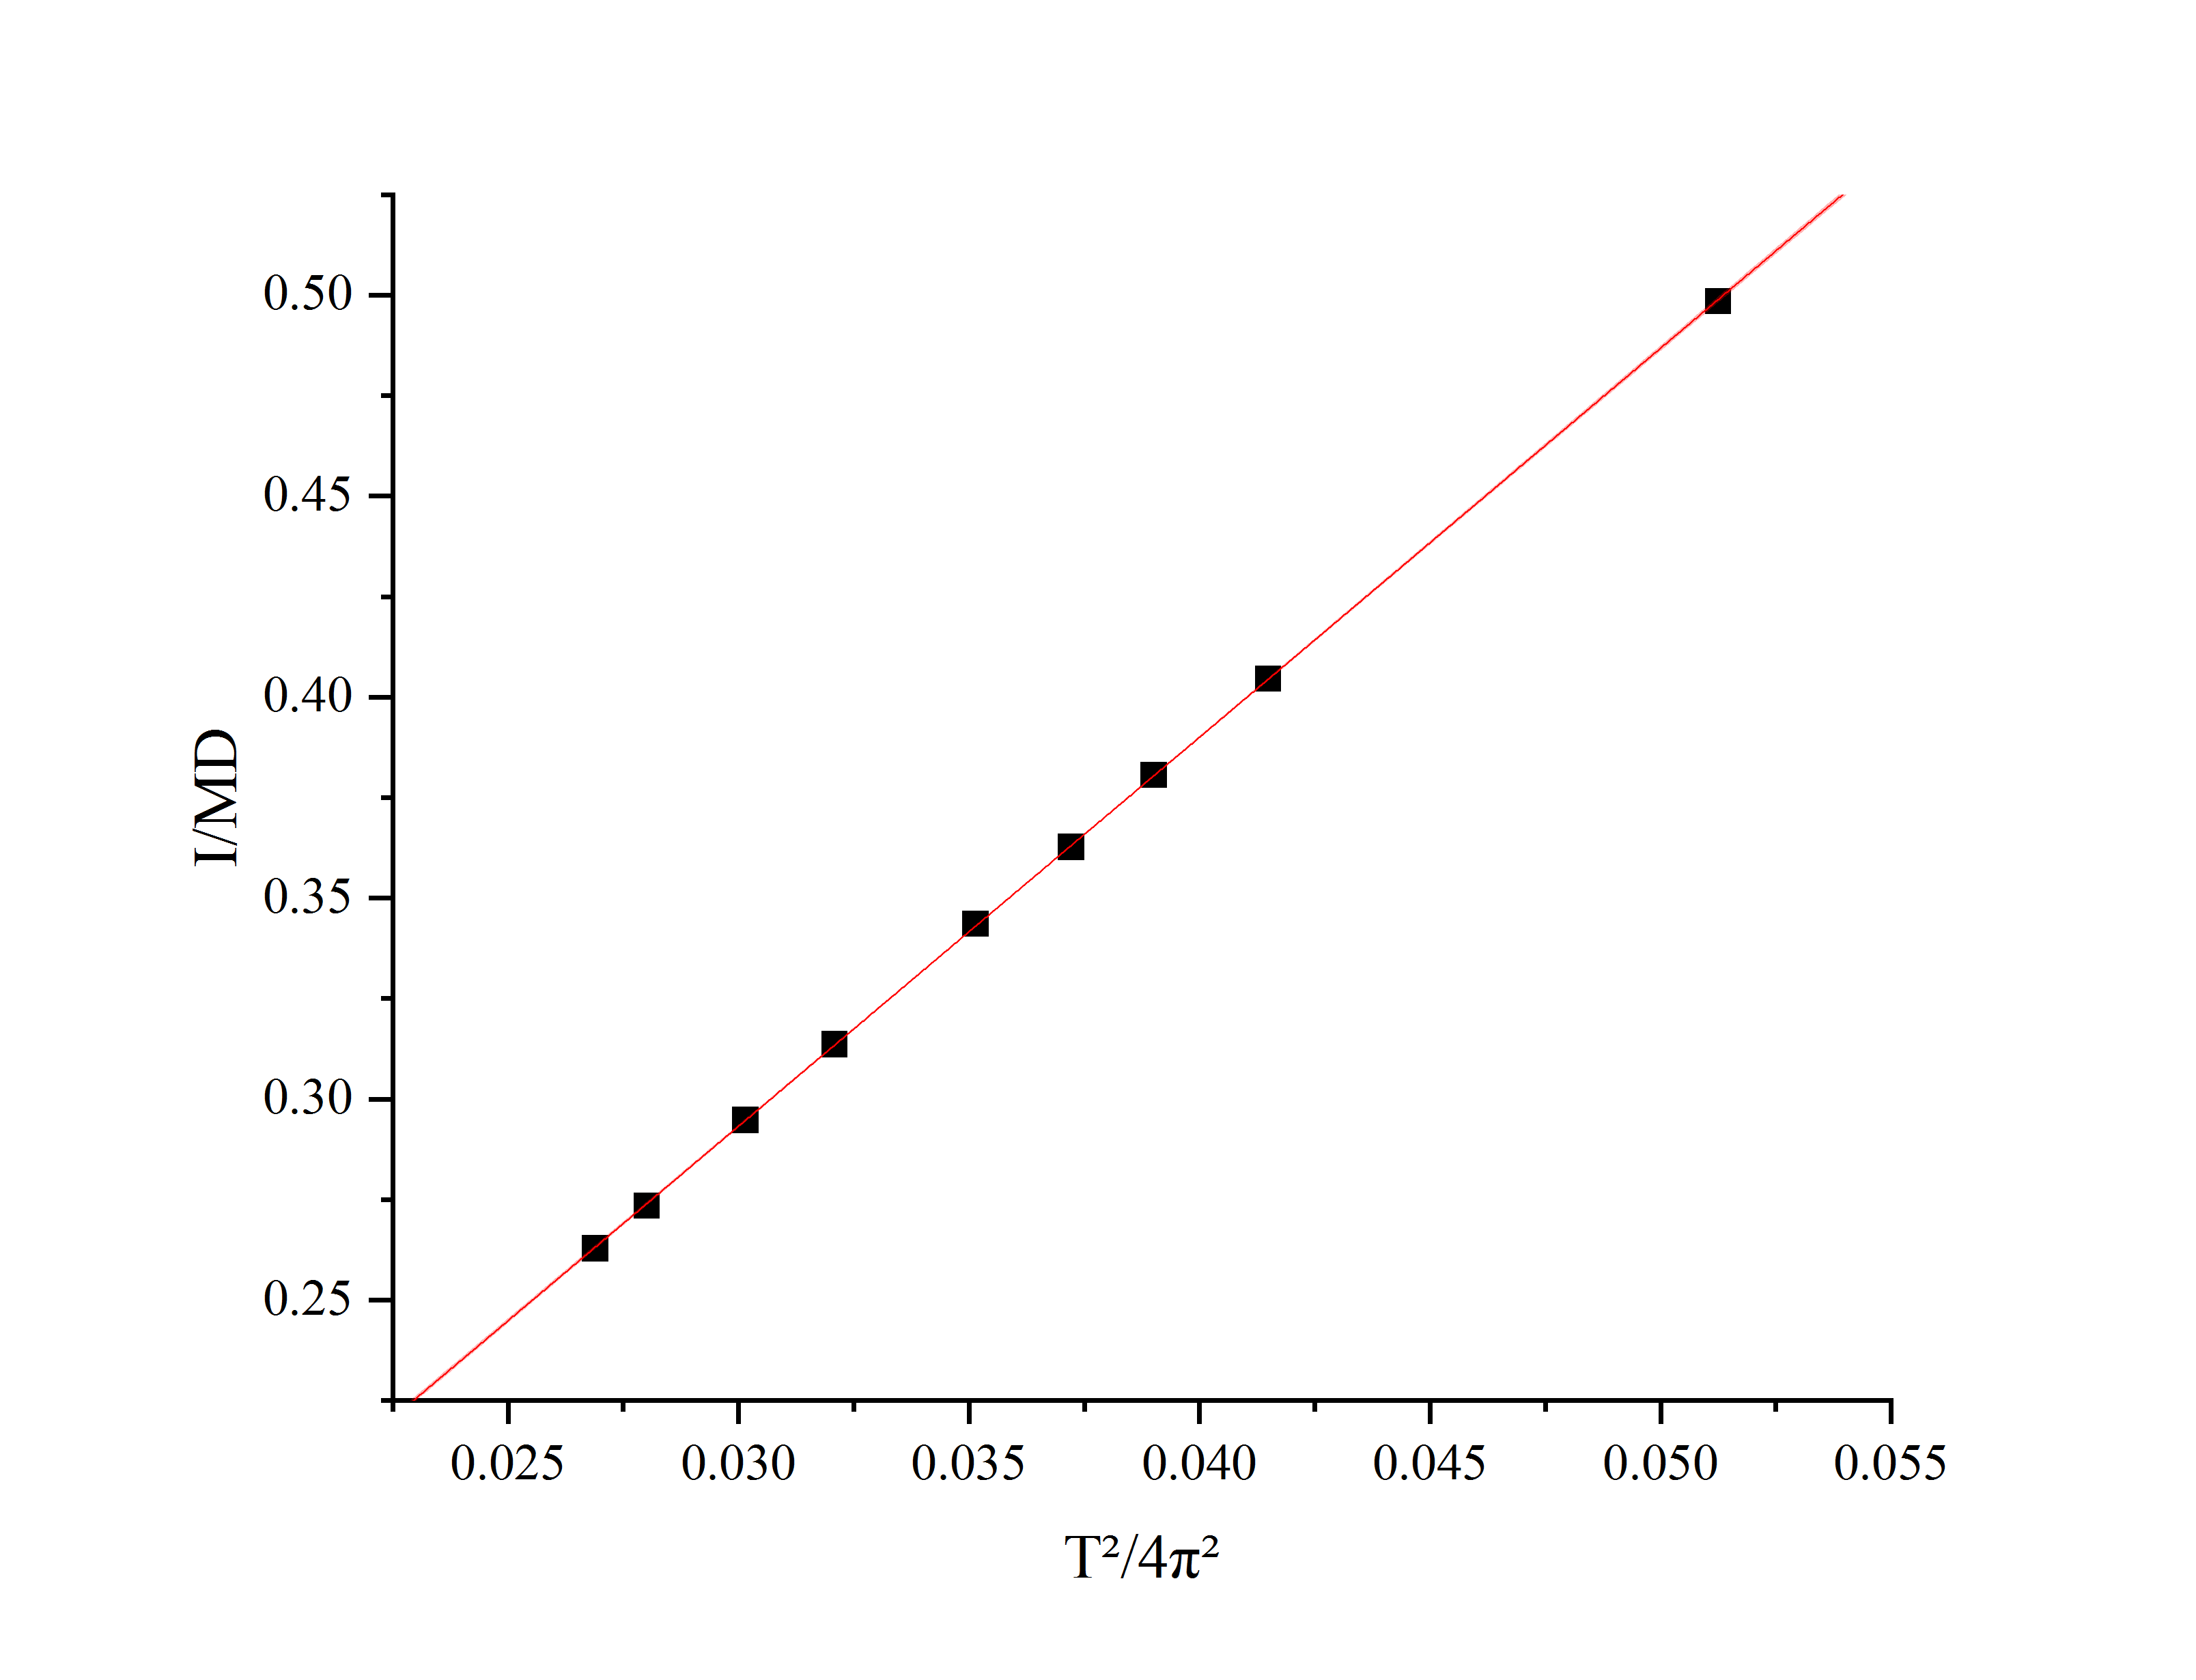
\includegraphics[trim={2cm 1cm 2cm 2.1cm},clip,width=\textwidth]{img/regressione.png}
\end{figure}

I risultati della regressione lineare sono i seguenti:
\begin{itemize}
  \item Intercetta $= (0.003 \pm 0.005)\;\unit{m}$
    (compatibile con $0$)
  \item Coefficiente angolare $g = (9.68 \pm 0.13)\;\unit{m\per s^2}$
\end{itemize}
Ricordando che $g_\text{atteso} = \qty{9.805}{m\per s^2}$,
possiamo affermare che $g_\text{misurato}$ risulta compatibile con
il valore atteso e, di conseguenza, l'esperienza ha avuto successo.

\pagebreak
\subsection{Misura dello smorzamento}

\emph{
  In questa sezione, illustreremo come il gruppo di lavoro abbia
  valutato lo smorzamento del moto e quanto questo sia significativo,
  prendendo come esempio la configurazione $\Gamma=\left\{\right\}$,
  dove il pendolo fisico è composto solamente da asta e rotore, senza
  l'aggiunta di cilindri.
}

\emph{
  Il gruppo di lavoro ha effettuato gli stessi passaggi per tutte le
  altre configurazioni: i risultati saranno messi in evidenza alla
  fine della sezione.
}
\vspace{2mm}

Sempre applicando la seconda equazione cardinale della dinamica,
è facile ricavare l'equazione differenziale che caratterizza il moto
del sistema sotto l'effetto delle forze di attrito.
Approssimando, come prima, $\sin(\theta)\simeq\theta$, si ottiene:
\[ \ddot{\theta} = -\lambda\dot{\theta} -\frac{Mg\,r_\text{CM}}{I_z^\text{\,tot}} \theta \]

dove $\lambda$ è una costante legata allo smorzamento del moto.
Le soluzioni di questa equazione differenziale sono infatti della forma:
\[\theta(t) = \theta_0\cos(\omega t)\,e^{-\lambda t}\]

dove la pulsazione del moto, $\omega$, è data da:
\[
  \omega^2 = \omega_0^2 - \lambda^2
  \qquad\text{con}\qquad
  \omega_0 = \sqrt{\frac{Mg\,r_\text{CM}}{I_z^\text{\,tot}}}.
\]

\begin{center}
    \begin{figure}[H]
        % trim={< v > ^}
        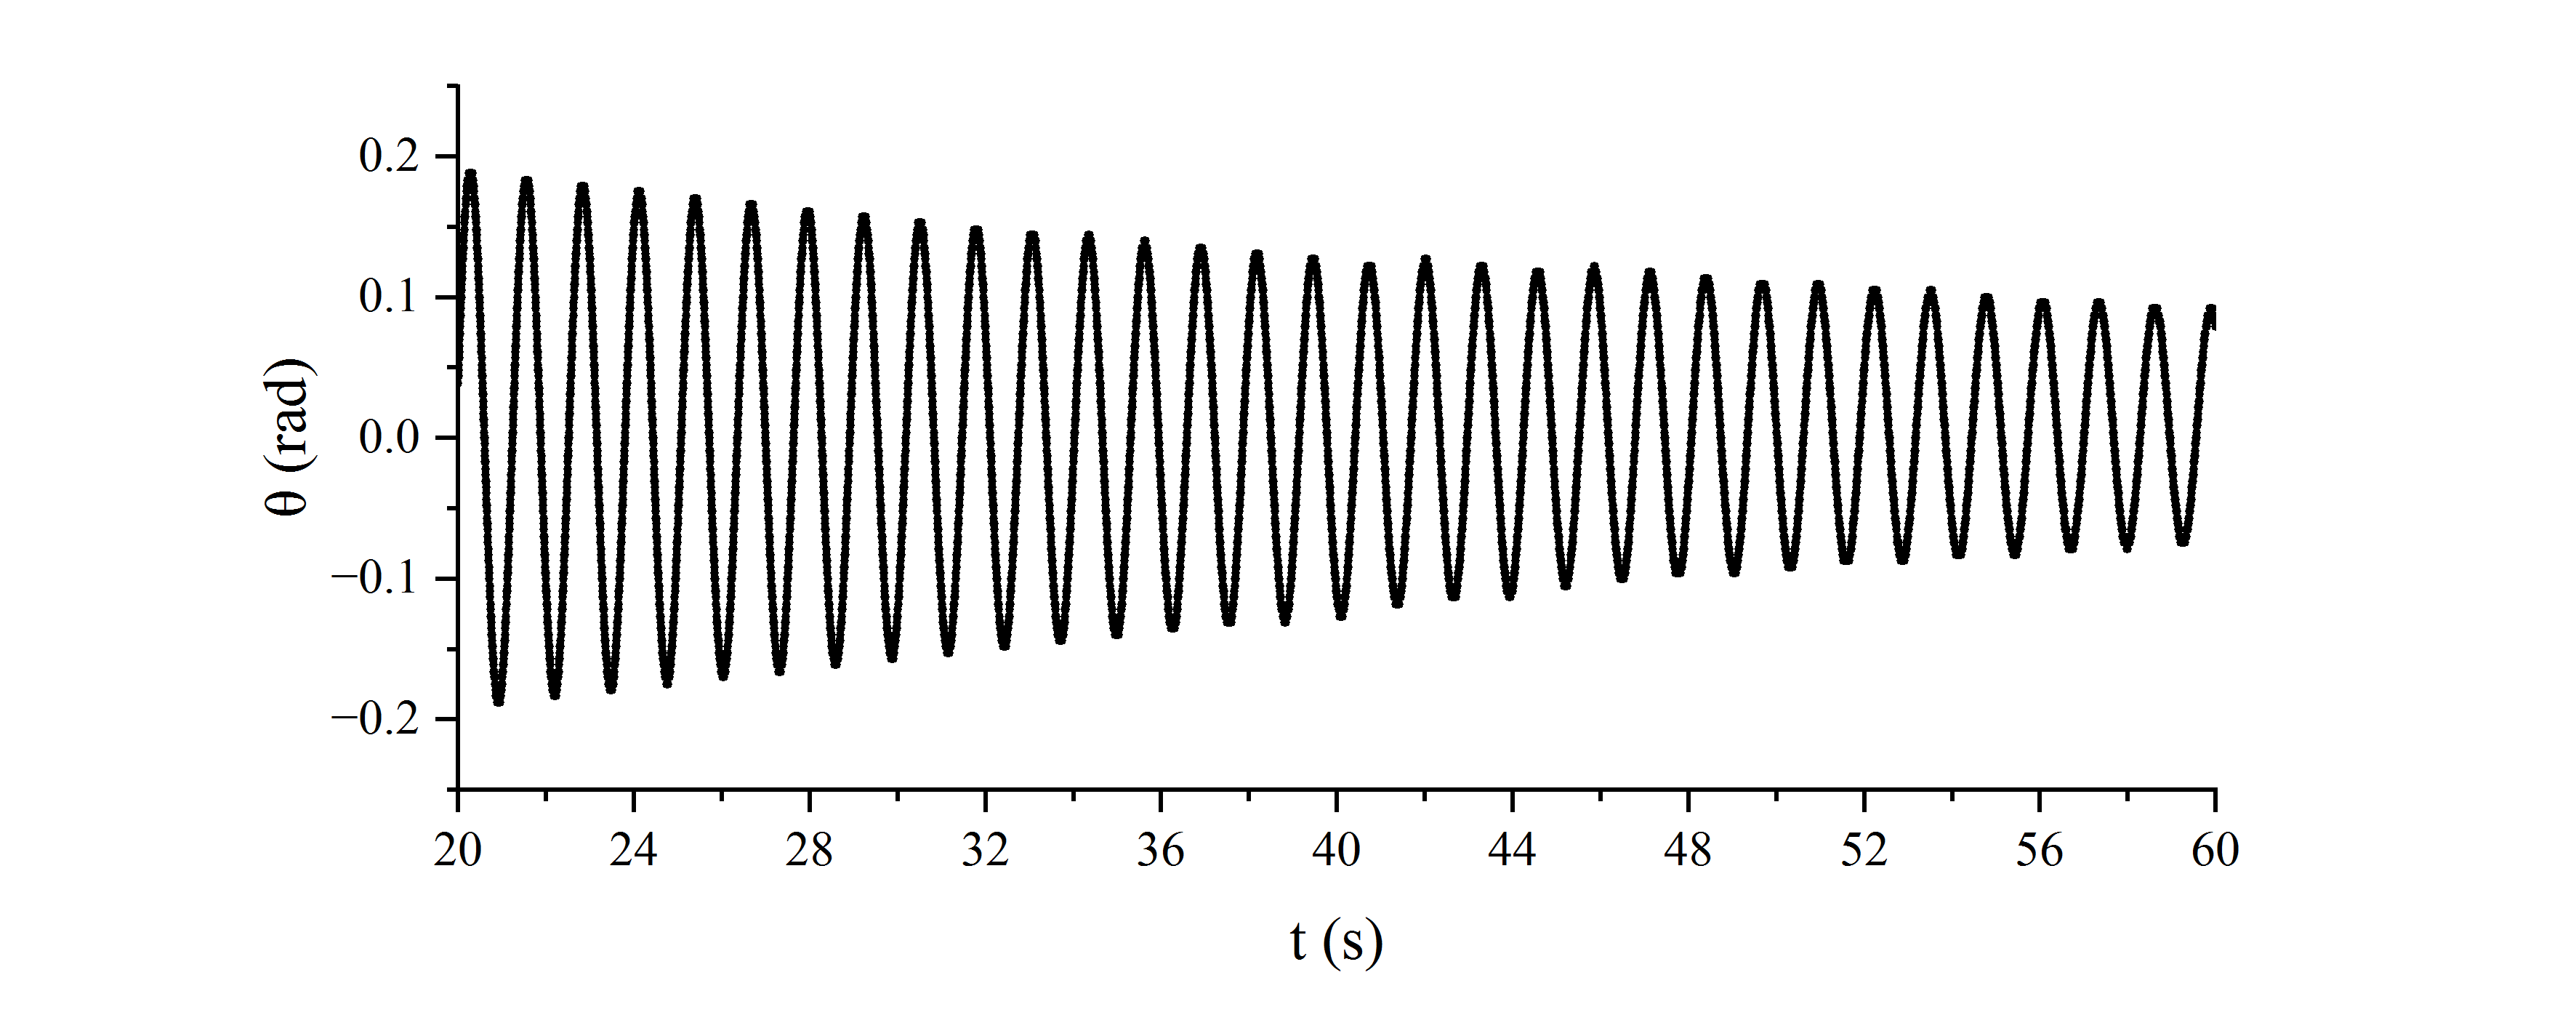
\includegraphics[trim={2cm .5cm 2cm .5cm},clip,width=\textwidth]{img/Graph1.png}
        \caption[]{\emph{
            Parte dei dati di un'acquisizione di $\theta(t)$
            con $\Gamma=\left\{\right\}$,
            come raccolti dal sensore di rotazione,
            riportati su una larga scala temporale.
            Si può chiaramente notare lo smorzamento
            del moto.
        }}
    \end{figure}
\end{center}

\pagebreak
Per stimare $\lambda$, il gruppo di lavoro ha proceduto come segue:
\begin{enumerate}
  \item
    Per prima cosa, abbiamo individuato i massimi dei nostri dati,
    ovvero gli insiemi di punti della forma
    $\left\{t_i,t_{i+1},\dots,t_j\right\}\times\left\{\theta_k\right\}$
    tali che $\theta(t_{i-1}) < \theta_k > \theta(t_{j+1})$.
  \item
    Per ogni massimo, ne abbiamo calcolato il punto medio,
    prendendo come $\delta t_\text{picco}$ la semidispersione $\frac{1}{2}(t_j - t_i) + \delta t$.
  \item
    Infine, abbiamo graficato i punti così trovati
    su scala logaritmica e
    abbiamo effettuato una regressione lineare (pesata\footnote{
      $\delta\!\ln{\left|\theta\right|}$, infatti, varia molto,
      nonostante $\delta\!\left|\theta\right|$ sia costante:
      ciò è conseguenza della propagazione degli errori.
      È inoltre possibile osservarlo nella \emph{Figura 2}.
    })
    sulle nuove ordinate. Il coefficiente angolare di tale
    regressione dovrebbe essere proprio $-\lambda$.
  \item
    Abbiamo ripetuto i tre punti precedenti sugli stessi dati,
    con $\theta$ cambiato di segno: così facendo, ai massimi
    si sostituiscono i minimi e tutto il resto dell'analisi
    è analoga. Per ogni configurazione abbiamo pertanto ottenuto
    due diversi valori di $\lambda$: $\lambda_\text{min}$ e
    $\lambda_\text{max}$. Abbiamo scelto di porre
    $\lambda=\frac{1}{2}(\lambda_\text{min}+\lambda_\text{max})$.
\end{enumerate}

\begin{center}
    \begin{figure}[H]
        % trim={< v > ^}
        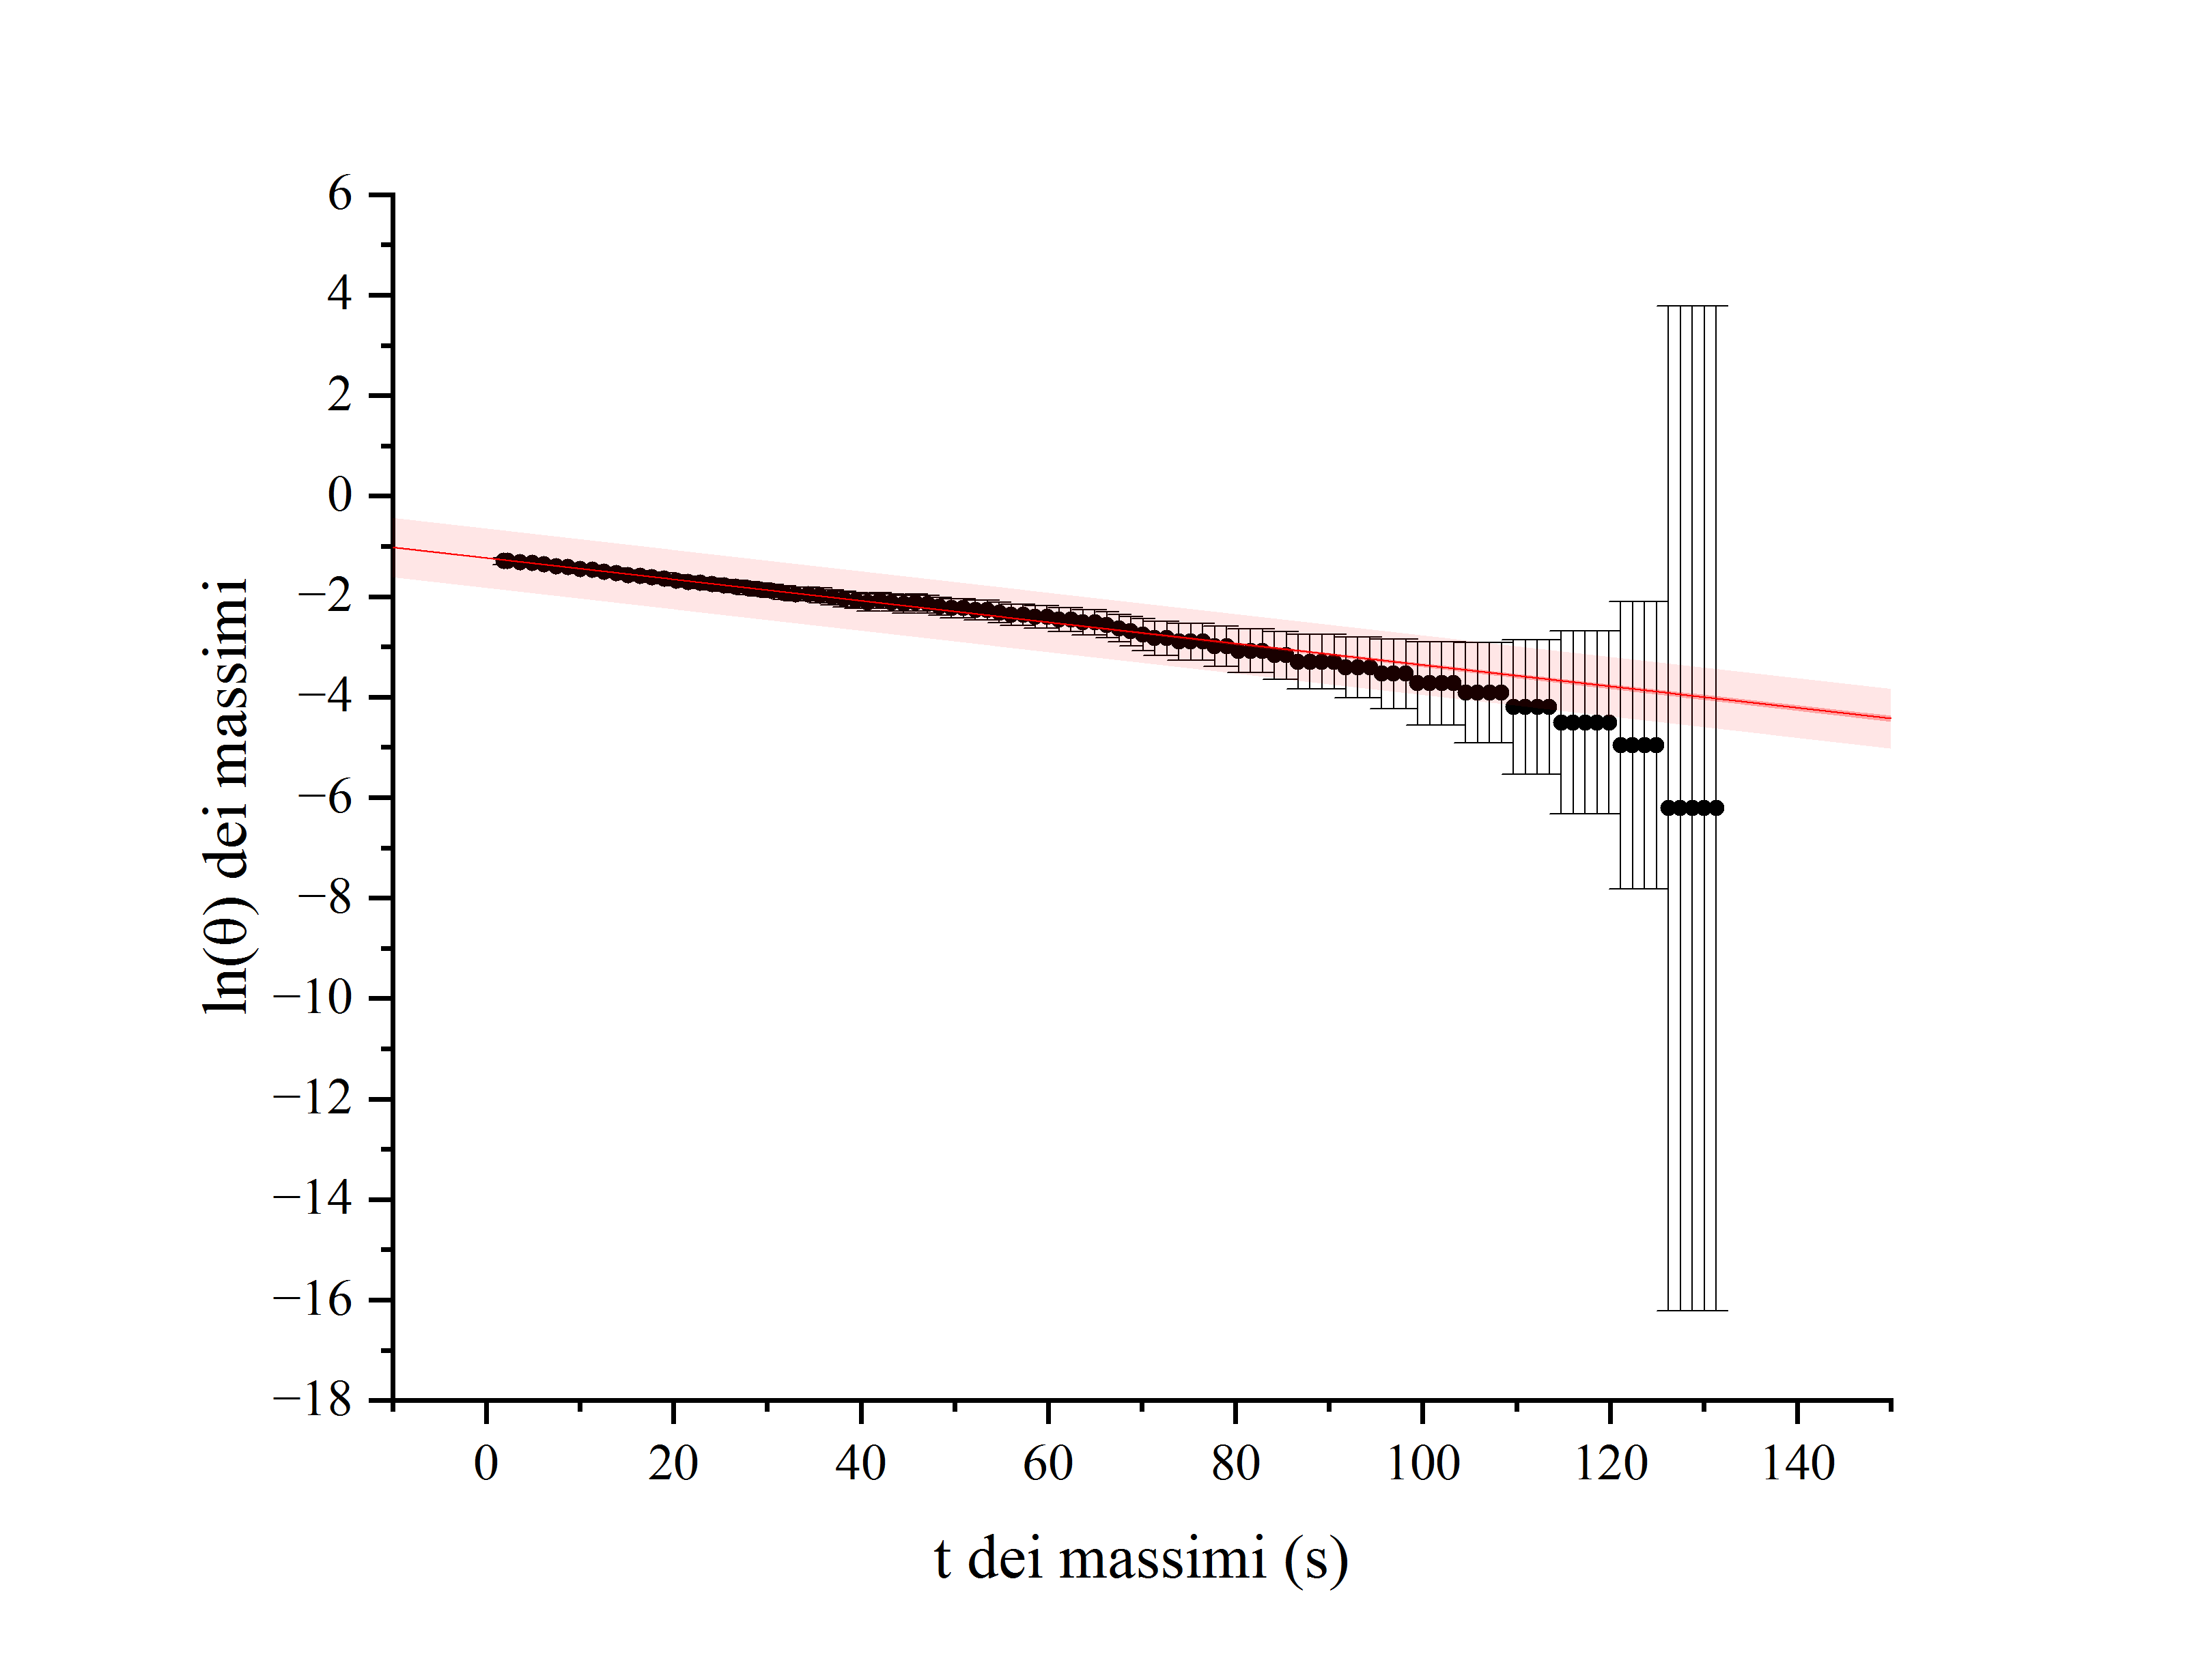
\includegraphics[trim={2cm 1cm 2cm 2.1cm},clip,width=\textwidth]{img/0max-exp.png}
        \caption[]{\emph{
            $\ln{\theta(t_\text{massimi})}$, su scala logaritmica.
            Sono riportate anche le barre di errore.
            In rosso, la retta di regressione lineare
            e in rosa la sua regione di incertezza.
        }}
    \end{figure}
\end{center}

Poiché l'obiettivo è calcolare $g$, la correzione da effettuare
sul periodo, per tenere conto dell'attrito, è la seguente:
\[
  T_0^2 = \frac{4\pi^2}{\omega_0^2}
    = \frac{4\pi^2}{\omega^2 + \lambda^2}
    = \frac{4\pi^2}{\frac{4\pi^2}{T^2} + \lambda^2}
    = \frac{1}{\frac{1}{T^2} + \frac{\lambda^2}{4\pi^2}}
\]

Effettuata questa correzione per ogni configurazione $\Gamma$,
si può allora costruire nuovamente una retta di regressione,
analogamente a quanto fatto nella sezione precedente.
La relazione fra le grandezze misurate, ricordiamo, è lineare:
\[ \frac{I_z^\text{\,tot}}{Mr_\text{CM}} = g \frac{T_0^2}{4\pi^2} \]

Riportiamo di seguito il grafico della nuova regressione,
unitamente ai risultati ottenuti.

\begin{figure}[H]
  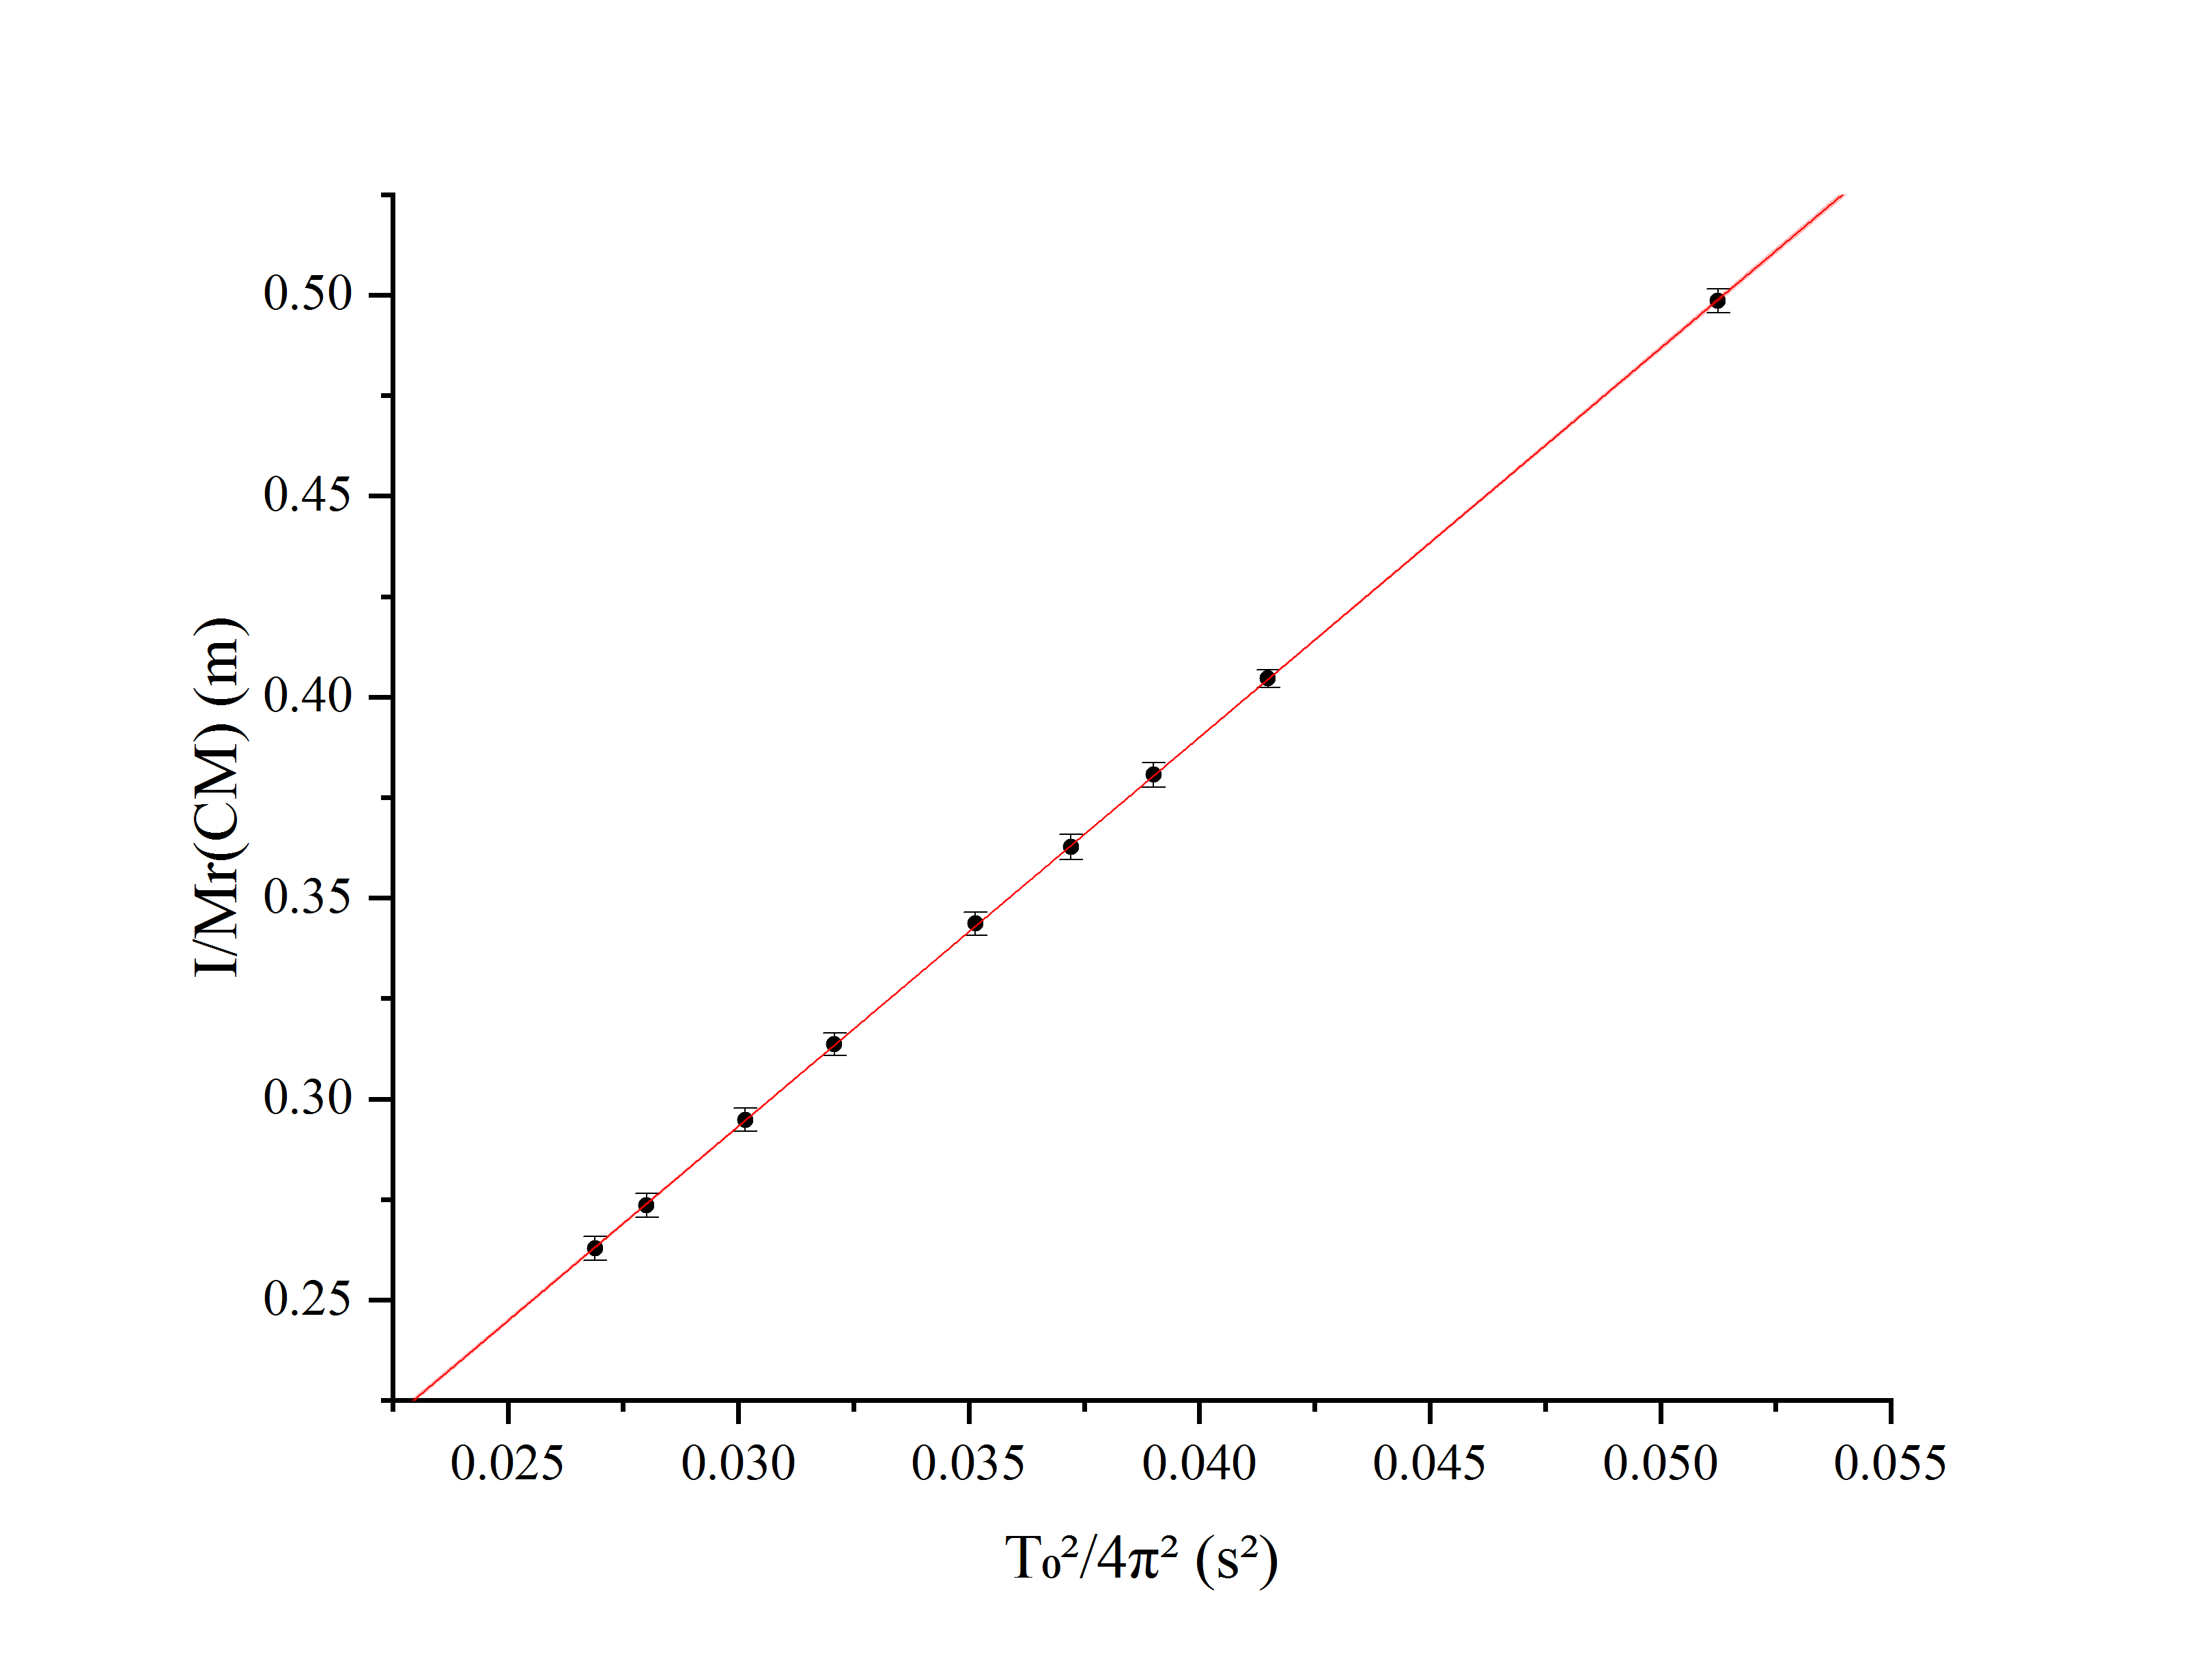
\includegraphics[trim={2cm 1cm 2cm 2.1cm},clip,width=\textwidth]{img/regressione-2.png}
\end{figure}

I risultati della regressione lineare sono i seguenti:
\begin{enumerate}
  \item Intercetta $= (0.003 \pm 0.005)\;\unit{m}$ (compatibile con $0$)
  \item Coefficiente angolare $g = (9.68 \pm 0.13)\;\unit{m\per s^2}$
    (compatibile con $g_\text{atteso} = \qty{9.805}{m\per s^2}$)
\end{enumerate}

Come è possibile osservare comparando questi risultati a
quelli precedentemente ottenuti, il valore di $g$ risultante
è rimasto essenzialmente invariato (al netto della sua incertezza).

In conclusione, possiamo affermare ragionevolmente che,
rispetto alla sensibilità degli strumenti di misura,
il contributo dell'attrito è trascurabile.

\end{document}
